% Chapter Template

\chapter{Related Work} % Main chapter title

\label{Chapter3} % Change X to a consecutive number; for referencing this chapter elsewhere, use \ref{ChapterX}

%----------------------------------------------------------------------------------------
%	SECTION 1
%----------------------------------------------------------------------------------------
\section{End-to-End Framework Optimizations for Deep Learning Accelerators}
There exist many end to end deep learning frameworks that allow
high level DSL programmers to create models that will be optimized to run
on a given hardware. Because of the diversity of hardware architectures that
must be supported and different types of memory layouts, frameworks must 
apply hardware agnostic optimizations before the backend creates architecture
specific kernels to cover general and repeated issues. In order to do this,
most frameworks implement their own unique model representation forms such
as specialized IR to enable the specific optimizations a framework can apply.
We discuss a survey of general memory focused optimizations that have been
developed by frameworks in this section.

\subsection{IR based Optimizations}
DLVM \cite{DLVM} (Wei et al. 2018) lowers a model into a domain specific IR
such that modern compiler optimizations could be performed on the operations
and simplified before LLVM IR is code generated for a backend to create
individual kernels. Deep learning compilers \cite{tensorflow} \cite{torch}
prior to this work would take a computational graph of operations and use off
the shelf vendor provided kernels to implement them. While the kernels
themselves are highly tuned, further optimizations could be made such as
algebra implication, kernel fusion, and other modern compiler techniques such
as dead code elimination and sub expression elimination could be applied to
further increase performance. By reducing the amount of operations needed to be
applied by analyzing which linear algebra operations could be simplified and
applying further parallelization optimizations once it is lowered into LLVM IR,
DLVM is able to minimize the amount of data transfer needed for kernels and how
much data is needed to run the kernels themselves.

After DLVM, Cyphers, Bansal, et al. 2018 at Intel created nGraph \cite{nGraph},
another IR based deep learning framework that takes an approach of using its
own IR. Instead of lowering a domain specific IR into LLVM after optimization
passes, nGraph takes the IR and passes it to a transformer, a code generator
that produces optimized backend code or code to be linked to a specific
backend's kernels. The goal was to create a more flexible IR that better supported
tensor based instructions and could be compiled in a more targeted fashion compared
to generic LLVM IR. Transformers also remove the dependency of backends having
to support LLVM.

\subsection{Graph based Optimizations}
TVM by Chen, et al. 2018 is a graph based end to end framework. 
TVM aims to create a framework that targets
multiple backends and accelerator architectures while still applying
fine grained optimizations for both intra and inter operator computations.
The main problem Chen et al. solved was the problem of existing deep learning
compiler frameworks only applying high level graph optimizations that did
not allow for tuning in operator specific implementations and left that to
the backends. However, the existing frameworks only supported a small handful
of GPU and CPU based backends. Creating support for new hardware backends
requires significant manual effort and there was no automated solution that 
existed. TVM allows for multiple backends to be supported while also
applying high graph level and operator implementation level optimizations
within its framework. Optimizations include operator fusion, SPM management via
operator rescheduling, pipelined memory access, and machine learning (ML) based
cost modeling for code generation. 
Operator rescheduling is the rescheduling of operators based
on data flow dependencies to maximize reuse by placing operators whose
inputs are outputs of another next to each other. Pipelined memory accesses are
when memory access instructions are executed without compute instructions having
been completed yet so that the next compute instruction does not need to wait
for the next memory instruction to complete. TVM also introduces an ML
based modeling method that estimates the performance cost of different
code generated and generates the lowest cost code to compile into the backed.
This means that the search space of parameters such as loop tiling size and 
loop unrolling factors are automated and decided based on the ML model.



\section{Scratchpad Memory Management Techniques}

\subsection{Graph Coloring}
Li et al. \cite{graphColoring} introduced the first approach to using graph coloring
as a scratchpad management technique to automatically and dynamically allocate data
structures like arrays in C programs. They partition the SPM space into pseudo-register
files so that the existing register based graph coloring allocator can be applied.
However, unlike scalar data in register based programs, array based data structures
contain longer live ranges or may not fit on the entire scratchpad. In such a case
the arrays are either tiled or arrays are split into sub-arrays such that the 
sub-arrays have different liveness with each other. This way, large arrays can
be accounted for in smaller chunks to fit on the SPM. 

\subsection{Integer Linear Programming}
Verma et al. \cite{verma} introduce an ILP approach to the same register
allocation problem for single dimensional arrays as the work Li et al. extend
for DNNs. Verma et al. reformulate the graph coloring problem into an ILP form
where constraints are added to ensure that tensors with overlapping lifetimes
are not allocated the same partition. The objective function is created to
maximize the number of data transfers saved. By using an ILP model over a
greedy algorithm, an optimal solution can be found. However, again, this
approach is not trivial to apply towards large variable tensors in DL workloads
due to assumptions the model takes of fixed size psuedo-registers and single
dimensional arrays.

% many core architecture
The problem of using more than one SPM is an issue that has mostly been ignored
until the work of Tao et al. 2021 \cite{manyCore} where they solve for an optimal data size
granularity to transfer between scratchpads and main memory to maximize performance
using a linear programming model for multicore architectures. The paper achieves
this via compiler-directed SPM data transfer model to formulate an allocation
scheme in a heterogeneous many-core architecture and then use the same allocations
to determine the optimal data transfer granularity to maximize performance.
The data transfer granularity is solved using ILP.

\section{End-to-End Framework SPM Management Optimizations for DLAs}

IBM's OnSRAM (Subhankar, et al. 2022) introduces the notion of two types of
runtime performance optimizations that can be done on computational graphs:
intra-node and inter-node optimizations \cite{onsram}. Intra node optimizations
are those that are focused on optimizing the operation kernel that the node
specifies. This means tiling in favorable sizes and across specific dimensions,
loop ordering, and DMA pipelining between tiles \cite{aladdin}.
Inter node optimizations are optimizations concerning the overall structure 
of the graph and the relationship between node connections. This includes
operator fusion and node reordering\cite{onsram}. In this section, we discuss
intra-node and inter-node optimizations specific to SPM management for DLAs.

\subsection{Intra-node SPM Management Optimizations}
% Toplib
Li et al. 2020 introduced TOpLib \cite{toplib}: a compiler-assisted operator
template library for DNN accelerators that focused on automated kernel
generation with optimized memory management using graph coloring. TOpLib builds
on the graph coloring solution to the register allocation problem applied to
SPM management for embedded devices but for DNNs. The key difference is that in
non-DL workloads, allocations are targeted for single dimensional arrays whose
sizes are known statically. Meanwhile, for DL workloads, tensors are high
dimensional, variable sized, and can often be larger than the size of the SPM
itself.  This requires an approach to dynamically partition the SPM into
variable sized psuedo-registers rather than equal sizing. The general concept
that they apply is as follows. A static walk through of kernel code for a given
operator is applied to analyze the liveness of each tensor used within it.  The
liveness of each tensor can then be used to create an interference graph of
tensors where tensors on an interference graph have overlapping lifetimes.
This graph can then be used to apply a graph coloring strategy to cluster
tensors with non-overlapping lifetimes onto the same partition of the SPM,
while overlapping lifetimes will be allocated separate partitions. The paper
proved that such an automated solution reached close to or exceeded hand
written assembly kernels and reach on average a 90\% speed up over
non-optimized kernel code.  While this approach could have been generalized to
the overall DNN case from the kernel case, this work applies a different
approach similar to the work presented by Verma et al. 2004 using an ILP model.
However, Li et al. demonstrate that a greedy graph coloring approach can reach
close to optimal performance across a multitude of operators.

\begin{figure}[thb!]
\centering
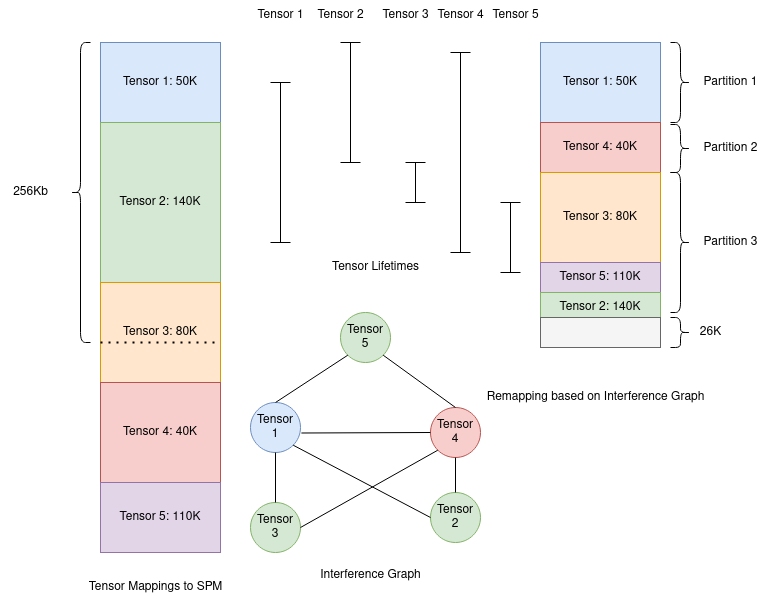
\includegraphics[scale=0.5]{Figures/graph_coloring_example.png}
\decoRule
\caption[SPM Allocation Using Graph Coloring]{Example of graph coloring. Not all tensors can be
mapped to the SPM at the same time so an interference graph is created
based on their lifetimes and colored accordingly. The resulting mapping on the 
right contains partitions for tensors based on their lifetime and colors such that
all tensors fit on the SPM without contention.}
\label{fig:graph_color}
\end{figure}

Figure \ref{fig:graph_color} shows an example of how TopLib \cite{toplib} uses
a graph coloring register allocation strategy to fit intermediate tensors onto
a scratchpad in a kernel.


\subsection{Inter-node SPM Management Optimizations}
% on sram

Existing deep learning frameworks are not modular like modern programming
language compilers \cite{tensorflow} \cite{TVM} \cite{nGraph}. Differences in
supported operation and backends, optimization opportunities based on IR
structuring, and lack of a standardized IR \cite{nGraph}\cite{DLVM} all lead to
why frameworks tend to be standalone projects that have little interoperability
between layers of other compilers. Because of the fact that many of these
frameworks are built from the ground up, they tend to re-implement many
optimizations already explored in other frameworks for their own IR. In
addition to the major engineering efforts required to do this, frameworks also
implement their own IR for the sake of implementing their own unique kernel
optimizations. Thus, almost all research efforts for memory efficiency within
the deep learning framework space have been on intra-node optimizations
facilitated through custom IR transformations and code generation. In contrast,
OnSRAM exists as a interoperable compiler extension for computational graph
based compilers to apply internode optimizations to maximize SPM utilization.

%The motivation of such optimizations come from the minimization of memory
%transfers which speed up inference runs by up to 5.17x \cite{onsram}. OnSRAM
%exploits the repeating usage of outputs in a graph and identifies the outputs
%that can pinned to minimize memory transfers which decrease inference time and
%decrease energy costs. The ultimate performance gained from pinning outputs
%comes from multiple inference runs where the cost of mapping pinnable tensors
%are amortized by the time saved through iterative inference runs of the same
%model.

%Such inter-node memory management techniques occur due to the presence of
%inherent repeating patterns of operations to support deep learning
%architectures, including matrix multiplication and convolution operations.

OnSRAM achieves its goal of maximizing SPM utilization by analyzing inter-node
data-dependencies in computational graphs and using identified data reuse
opportunities to create an optimal data allocation scheme for on-chip memory of
the target DLA. OnSRAM shows that there exists a potential of up to 5.2x
speedup opportunity for DL inference after integrating their SPM management in
the runtime of Tensorflow \cite{onsram}.


% TODO: graph node reuse opportunities explained
% TODO: explain what pinning (avoids incurring data transfer costs)
% TODO: graph figure

% re-explain static graphs
% how dnn graph structures create reuse oppurtunities
% how reuse oppurunities translates into pinning model
% how Onsram actually does the allocations and pinning

% "effective management of the on-chip SPM across the nodes or layers of a DNN,
% i.e., retaining the activations produced by a given layer on the on-chip
% scratchpad so as to eliminate writes/reads to/from external memory when they
% are reused in subsequent layers. "

% Inter-node SPM management is relatively easy in the context of earlier DNN
% topologies which were sequential in nature (e.g., AlexNet and VGG), i.e., with
% every layer connected only to the layer succeeding it. In such cases, the
% output activation of each layer (if fits) is held on-chip for one additional
% step during which it is consumed and discarded. However, two recent trends in
% modern DNN research make this an interesting and challenging issue.  — Complex
% Topologies. Recent DNN topologies such as ResNets [38], Inception [28],
% DenseNet [43], Multi-Head Attention [90], Neural Architecture Search (NAS)
% [104] and others rely on complex connections across layers (e.g., re-convergent
% paths) to achieve superior accuracy. Such topologies require
% sophisticated management of the finite on-chip memory, balancing the tradeoffs
% between the benefits of improving reuse by retaining acti- vations on-chip vs.
% sacrificing reuse on other activations due to capacity limits.

% Based on these observations, we propose OnSRAM, a compiler extension that
% integrates within DL frameworks to manage the on-chip memory of AI
% accelerators for the end-to-end application.  Without burdening the end-user
% to manage the SPM, based on the hardware parameters and constraints, OnSRAM
% provides hardware-aware software optimizations to meet the memory bandwidth
% requirements across all the layers of the DNNs

As previously described, computational graphs consist of nodes that represent
operations and the edges represent data-dependencies between operations. During
execution, each operation is loaded from main memory by the host device into
the accelerator's SPM along with the operation's required weights and input
tensors. Each transfer of data between main and on-chip memory incurs DMA
transfer costs exacerbated by the bandwidth of the bus. Similarly, when a DLA
executes an operation, the resulting output tensor is placed onto on-chip
memory and again transferred back to main memory. When two connected nodes,
ie. an output of one operation is the input of the next, are scheduled
sequentially, a reuse opportunity exists: the output tensor of the first
operation can be pinned on the SPM without being transferred back and used
immediately by the next operation, thereby eliminating unnecessary transfer
costs. OnSRAM creates an SPM management framework to minimize inference runs
by creating an optimal pinning tensors onto the SPM.

OnSRAM-Static, the static DNN graph based SPM manager is described as follows.
A graph of operations that represents a DNN is passed to OnSRAM-Static as an
input. All input and output data tensors of each node is analyzed for the start
time, end time, number of reuses, distance between reuses, and size of the
tensor. A weighted sum of these properties is calculated for each tensor to
determine a metric for the cost incurred should a tensor be saved back to main
memory and reloaded onto the SPM again. Based on the graph execution schedule,
the tensors are psuedo-sorted in cost order. They are psuedo-sorted since
tensors that do not overlap in their lifetimes do not need to be sorted relative to
each other. These sorted tensors are then considered in a greedy fashion where
tensors of the highest cost are considered for pinning first. Tensors are only
pinned if they can be pinned for the entire duration of their lifetime without
obstructing tensors needed for other operations before their next reuse. Figure
\ref{fig:onsram_stack} shows an overview of how OnSRAM fits as a compiler extension
into deep learning frameworks.

\begin{figure}[thb]
\centering
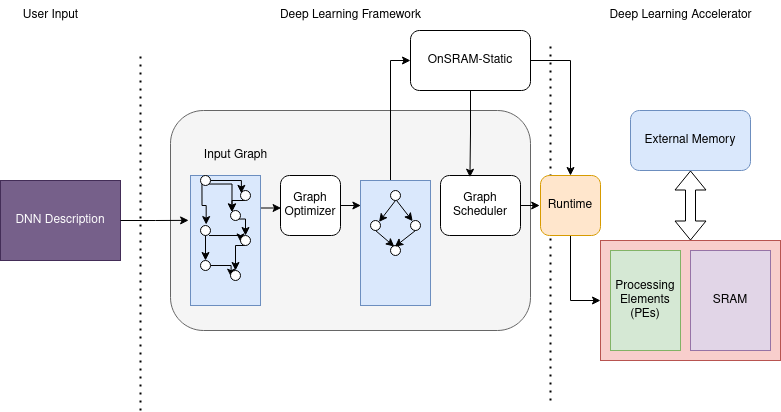
\includegraphics[scale=0.5]{Figures/onsram_stack.png}
\decoRule
\caption[Overview of OnSRAM]{Overview of OnSRAM}
\label{fig:onsram_stack}
\end{figure}


OnSRAM-Static only applies to input and output tensors, not weights. This is
due to the fact that weights are single use objects that are only needed for
the layers they are used in. There exists no reuse opportunity unlike output
tensors since all layers contain independently different weights. Thus, weights
are not considered for pinning for both OnSRAM-Static and our extension work as
well.

Another aspect that OnSRAM does not consider is applicability towards training.
The assumptions of the problem change when considering training and
significantly increase the difficulty and search space for an optimal solution.
This requires separate compiler extension implementations to be designed into
separate portions of the framework. Further, batched training, partitioned
accelerators, distributed systems, and large reuse distances due to backward
passes and batched data \cite{onsram} bring significant design challenges that
are not present in inference. Thus we have also chosen not to extend this work
in this regard as well.


% IR based ones (ngraph and DLVM)
% simplify shit to remove unnessary datamovement by creating smaller or fused
% kernels so that you don't have to have to jam together a bunch of complex
% kernels to complete your dataflow. 
% graph based ones (smaug and TVM)

